%==========================================================================
% BEGIN #3 - ESPECIFICAÇAO/MODELAÇAO DO SOFTWARE
% Apresentação, descrição e representação dos vários elementos e serviços a serem implementados no projeto, utilizando-se, se possível, uma exposição orientada ao serviço suportada por representações UML num nível de abstração adequado.

\newcommand{\headercaso}[5]{
    \subsubsection{#1}
    \textbf{Descrição:}
    \begin{itemize}
        \item[] #2
    \end{itemize}

    \textbf{Condições:}
    \begin{itemize}
        \item[] \textbf{(Pre)} #3
        \item[] \textbf{(Pos)} #4
    \end{itemize}
}


\newcommand{\normal}[2]{
  \textbf{#1} % Title
  \begin{enumerate}[label=\arabic*.] % Numbered list
    \foreach \x in {#2} {
      \item \x % Steps, split by delimiter
    }
  \end{enumerate}
}

\newcommand{\alt}[3]{
  \textbf{#1 - no passo #2:} % Title, number, and parent step number
  \begin{enumerate}[label=\arabic*.\arabic*] % Nested numbering
    \foreach \x [count=\i] in {#3} {%
      \item[\the\numexpr#2.\i\relax.] \x % Numbering and steps
    }
  \end{enumerate}
}

%==========================================================================

\chapter{Especificação e Modelação do Software}

    \section{Apresentação Geral da Especificação}

        De modo a dar resposta aos requisitos e facilitar a discussão sobre a plataforma com \textit{stakeholders} de nível técnico variado, recorreu-se à elaboração de casos de uso (e correspondente diagrama) para modelar o seu comportamento e a um diagrama de domínio para modelar a sua estrutura.

        Continuou-se aqui a codificação por cores alusivas aos componentes abstratos estabelecidos na maquete (figura \ref{fig:maquete}): azul para utilizadores, amarelo para encomendas, verde para modelos e violeta para peças/inventário.

    \newpage
    \section{Aspetos Estruturais}

         A modelação estrutural materializa-se com um diagrama de domínio. Teve o objetivo de fomentar o debate quanto à arquitetura do sistema, em termos de componentes temáticos e entidades conceptuais, e explicar como se relacionam uns com os outros numa perspetiva estática.

        \begin{figure}[h]
            \centering
            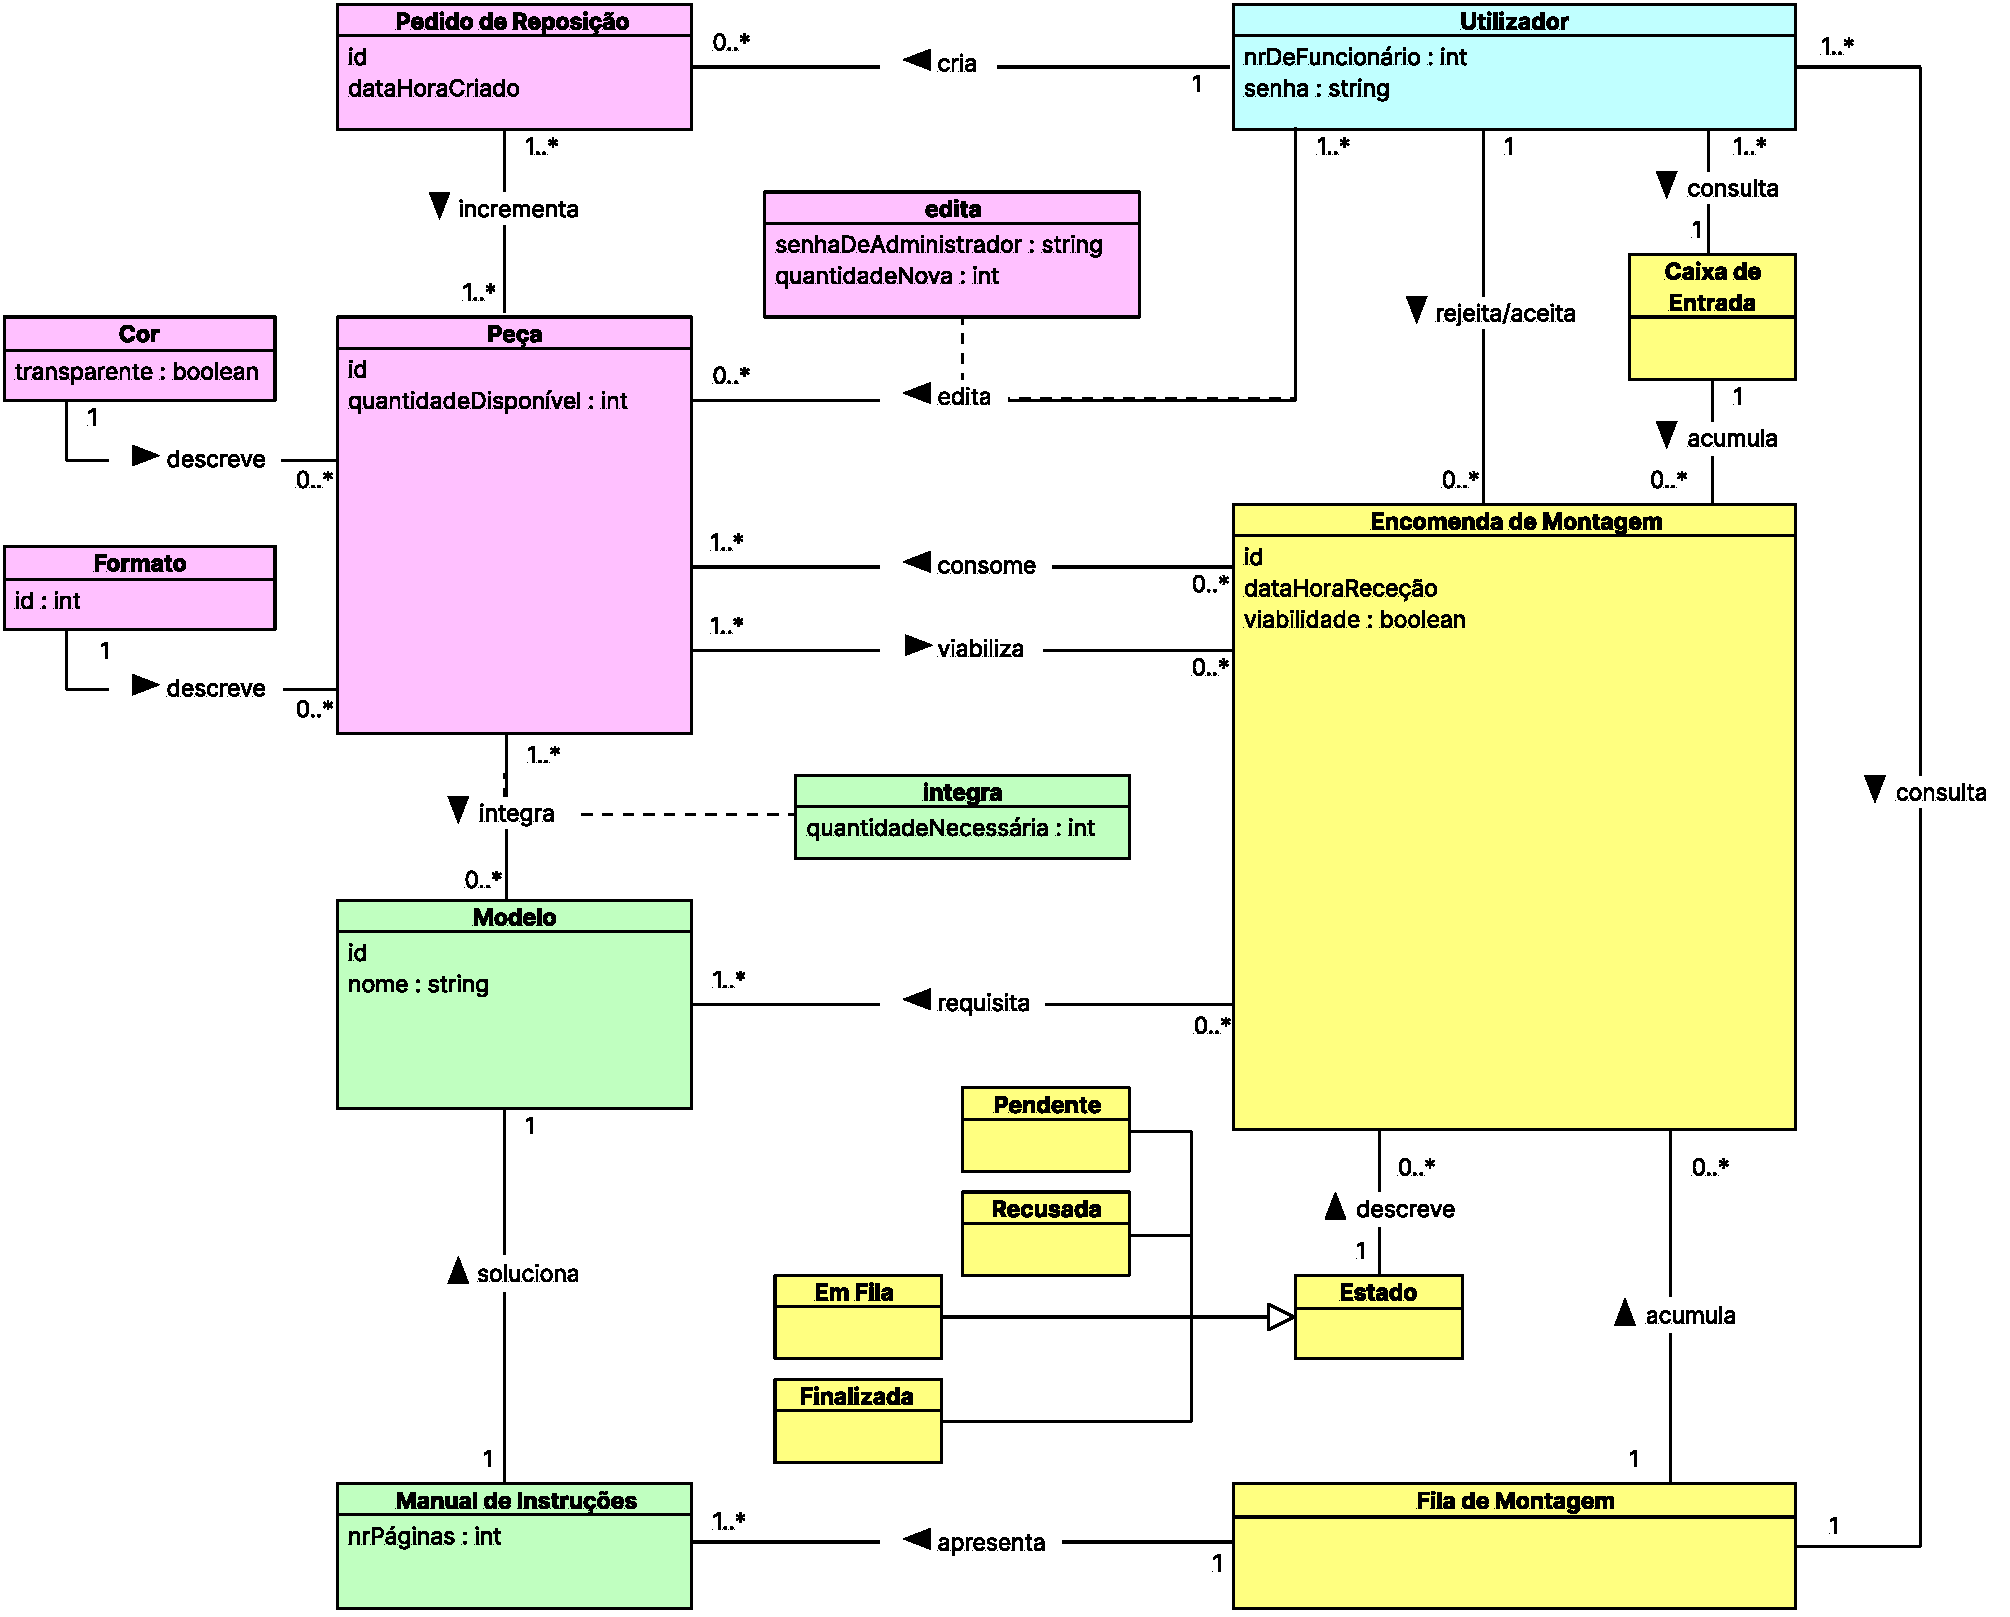
\includegraphics[width=1\textwidth]{images/cap3_diagclasses.pdf}
            \caption{Diagrama de domínio}
            \label{fig:diagclasses}
        \end{figure}

        \newpage
        \subsection{Utilizadores}

            O utilizador é caracterizado pelas suas credenciais de autenticação.

            \begin{itemize}
        
                \item \textbf{Utilizador edita Peça:} Ver requisito 2.4.4. Esta é uma operação fazível por um ou mais utilizadores. Na perspetiva oposta, a quantidade disponível de uma peça não se garante como tendo editada por qualquer utilizador.
        
                \item \textbf{Utilizador rejeita/aceita Encomenda:} Ver requisitos 2.3.3 e 2.3.4. Uma encomenda só é processada por um único utilizador. Enquanto isso, um utilizador pode processar entre nenhuma a múltiplas encomendas.
        
                \item \textbf{Utilizador consulta Caixa de Entrada:} Ver requisito 2.3.1. A consulta da caixa de entrada de encomendas só faz sentido ser realizada por um ou mais utilizadores. Tendo o propósito de colecionar as encomendas pendentes, só existe uma.
        
                \item \textbf{Utilizador consulta Fila de Montagem:} Ver requisito 2.3.5. Aplica-se o mesmo raciocínio do relacionamento anterior, mas orientado às encomendas em fila.
        
                \item \textbf{Utilizador cria Pedido de Reposição:} Ver requisitos 2.4.2 e 2.4.3. Um pedido de reposição vem a existir partido dum certo utilizador. Da perspetiva contrária, um utilizador pode criar quantos pedidos pretender, portanto, de zero a vários.

            \end{itemize}

        \newpage
        \subsection{Encomendas}

            Uma encomenda é caracterizada por um identificador, um registo temporal de receção e a sua viabilidade, esta última à mercê da presença de todas as peças necessárias. 

            \begin{itemize}
                \item \textbf{Fila de Montagem acumula Encomenda:} Ver requisito 2.3.5. A fila de montagem é uma entidade singular e universal com o propósito de colecionar encomendas, pelo que só existe uma e alberga de zero a múltiplas.
    
                \item \textbf{Estado descreve Encomenda:} O estado duma encomenda define se é apresentada no sistema (positivo caso Pendente ou Em Fila) e, se sim, se na Caixa de Entrada ou Fila de Montagem. Deste modo, cada encomenda tem obrigatoriamente um estado associado; da perspetiva oposta, um determinado estado pode estar a descrever entre zero a múltiplas encomendas em certo momento.
    
                \item \textbf{Encomenda requisita Modelo:} A empresa recebe encomendas que solicitam a montagem de um ou vários modelos. Da perspetiva oposta, um modelo específico pode ou não ser requisitado por quaisquer encomendas existentes. 
                
                \item \textbf{Encomenda consome Peça:} Como um modelo requer peças e a encomenda requisita vários modelos, o processamento duma encomenda (i.e. a colocação dela em fila) requer que sejam consumidas peças do inventário para a finalizar. Da perspetiva oposta, uma peça pode ou não ser consumida por quaisquer encomendas existentes. 
    
                \item \textbf{Fila de Montagem apresenta Manual de Instruções:} Ver requisito 2.3.6. Durante a conceção de cada modelo requisitado por uma encomenda posta em fila de montagem, é apresentado o respetivo manual de instruções. Assim, a fila de montagem é uma entidade singular que suscita a apresentação dos vários manuais.
        
            \end{itemize}

        \newpage
        \subsection{Inventário}

            Uma peça é inerentemente caracterizada por um identificador e uma quantidade disponível em inventário. Um pedido de reposição terá igualmente um identificador e também uma data/hora de criação.
        
            \begin{itemize}
                \item \textbf{Peça integra Modelo:} Um modelo LEGO é constituído por múltiplas peças, cada em quantidade necessária bem definida. 
    
                \item \textbf{Pedido de Reposição incrementa Peça:} Um pedido de reposição solicita incremento à quantidade de pelo menos uma encomenda. Na perspetiva contrária, a quantidade duma peça é incrementável por solicitação proveniente de múltiplos pedidos.
    
                \item \textbf{Cor/Formato descreve Peça:} O identificador duma peça é baseado no seu formato e cor. Assim sendo, valores específicos destas entidades podem descrever entre zero a múltiplas peças reconhecidas pelo sistema.
    
                \item \textbf{Peça viabiliza Encomenda:} Ver requisito 2.3.2. A viabilidade de conceção duma encomenda depende da existência em inventário das peças em quantidade necessária aos modelos requisitados. Assim, uma certa peça pode viabilizar de zero a múltiplas encomendas, dependendo dos modelos.
            
            \end{itemize}

        \subsection{Modelos}

            Um modelo tem um identificador chave e um nome correspondente.
            
            \begin{itemize}
                \item \textbf{Manual de Instruções soluciona Modelo:} Ver requisito 2.5.1. Cada modelo tem associado um manual de instruções que lhe é único.
            \end{itemize}

            

    \newpage    
    \section{Aspetos Comportamentais}

        \begin{figure}[h]
            \centering
            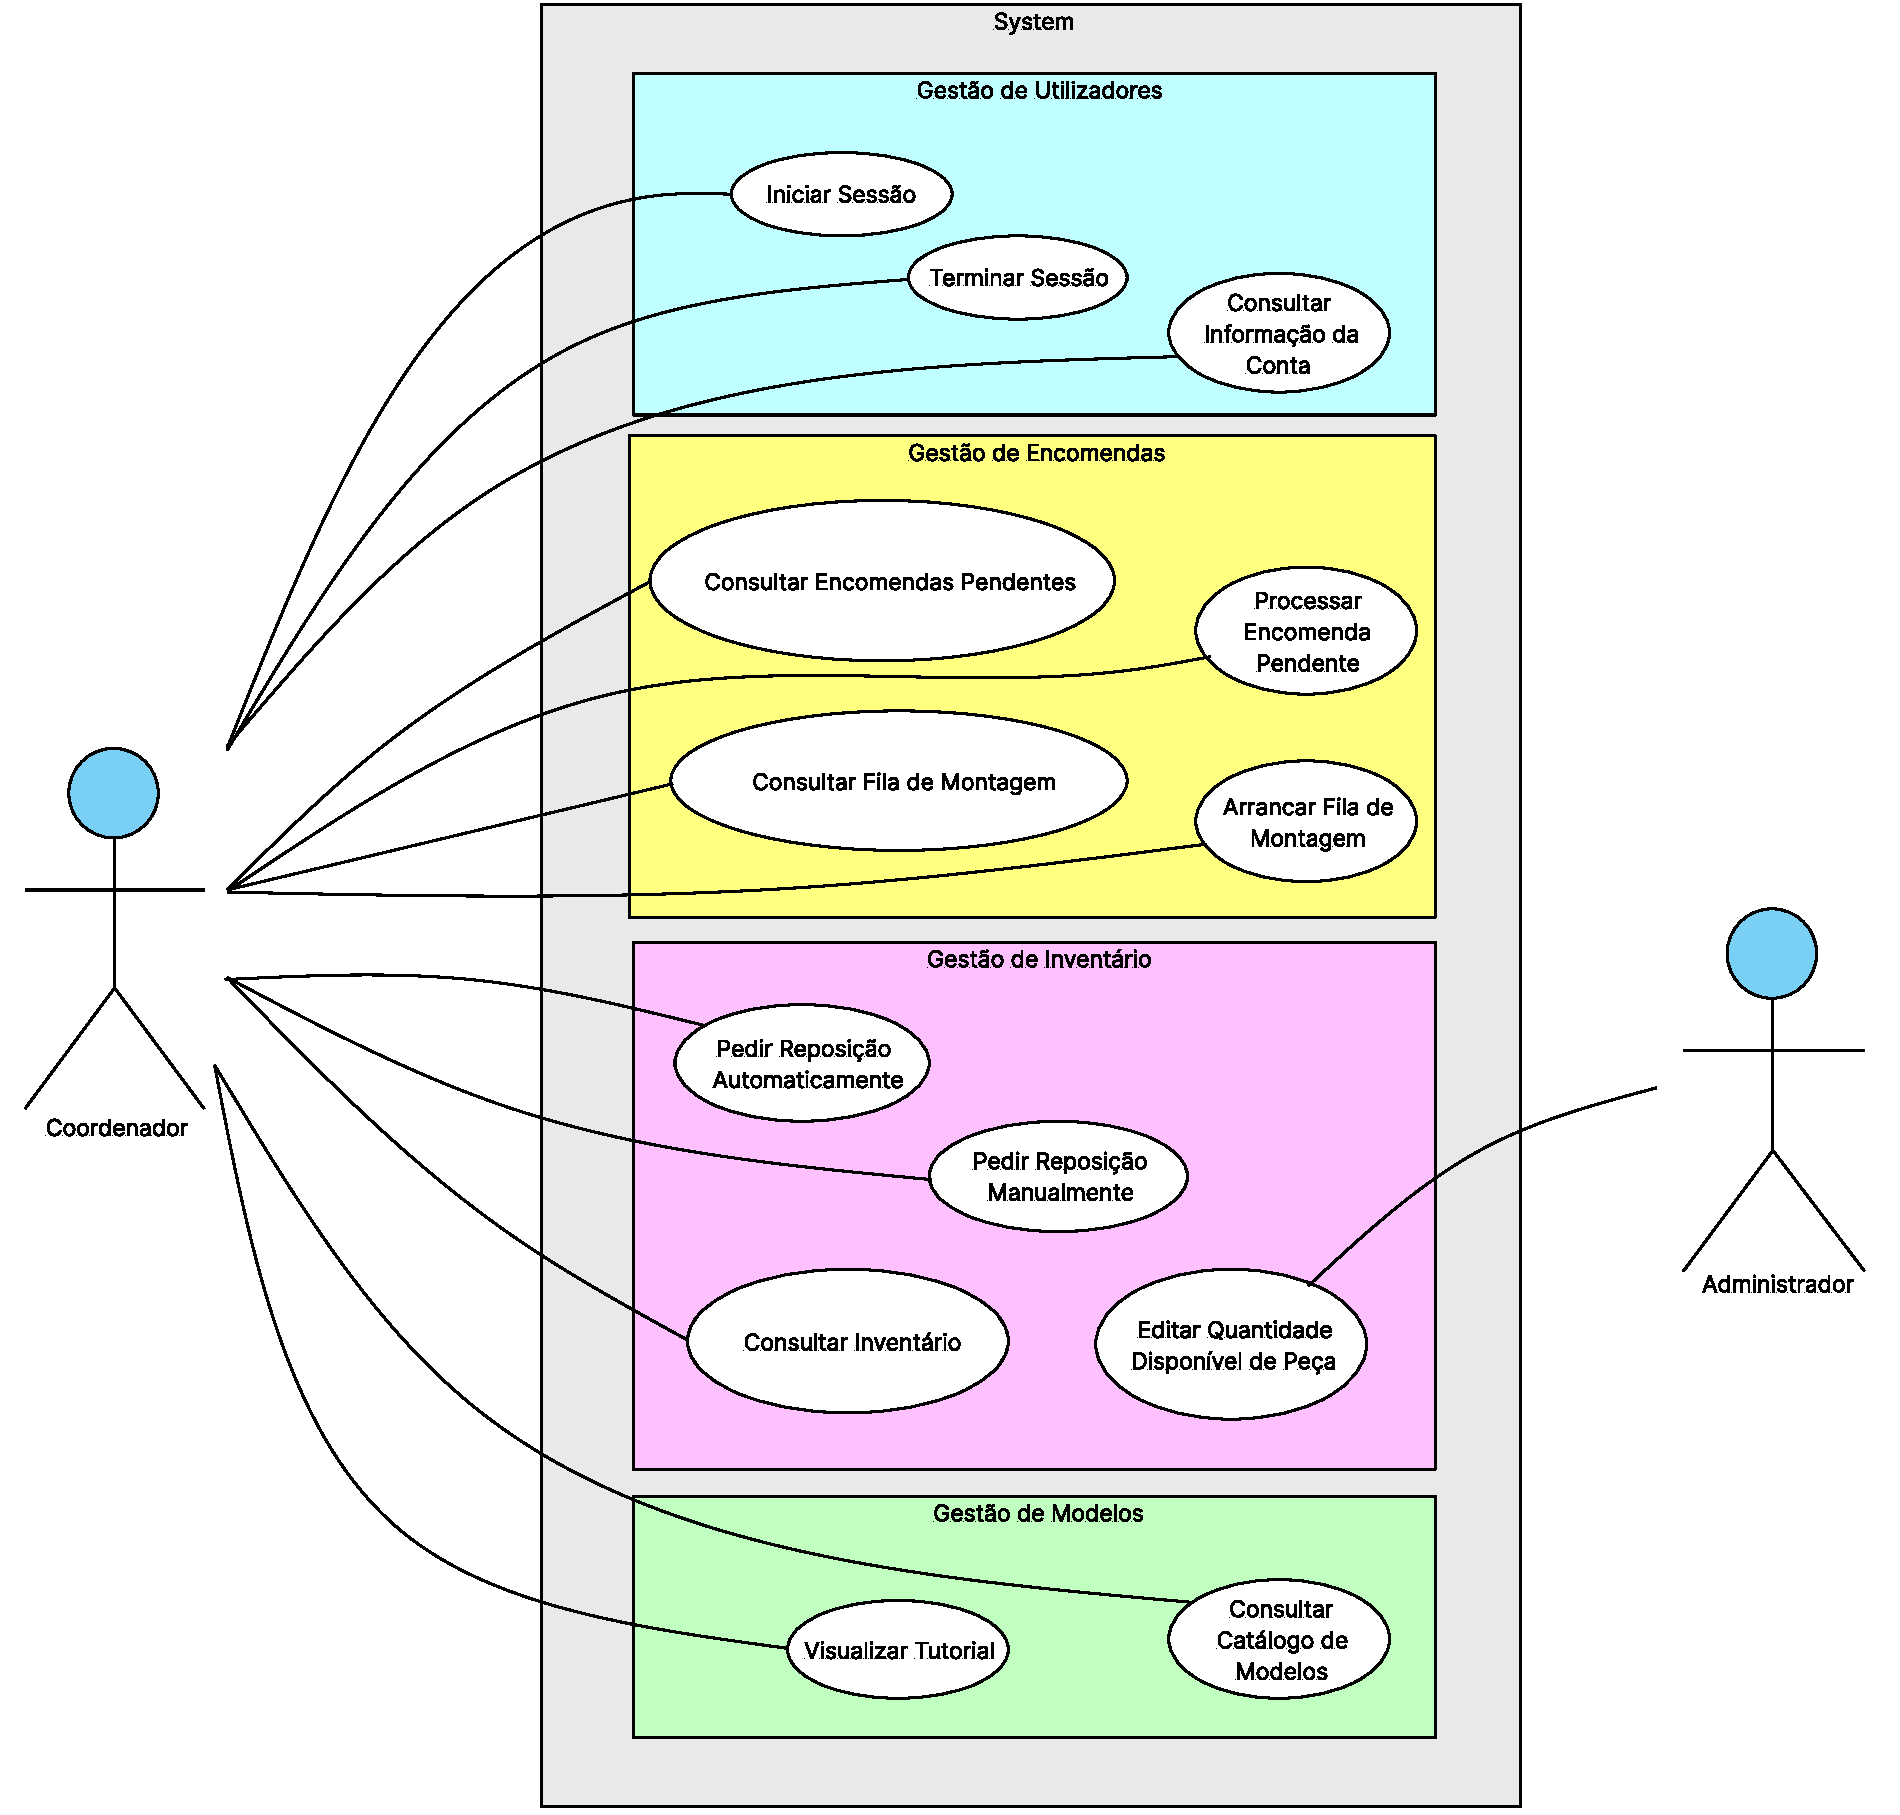
\includegraphics[width=1\textwidth]{images/cap3_diagcasos.pdf}
            \caption{Diagrama de casos de uso}
            \label{fig:diagcasos}
        \end{figure}
        
        %%%%%%%%%%%%%%%%%%%%%%%%%%%%%%%%%%%%%%%%%%%%%%%%%%%%%%%%%%%%%%%%%%%%%%%%%%%%%%%            
        %%%%%%%%%%%%%%%%%%%%%%%%%%%%%%%%%%%%%%%%%%%%%%%%%%%%%%%%%%%%%%%%%%%%%%%%%%%%%%%
        \newpage
        \subsection{Casos de Uso sobre Encomendas}

            \headercaso{Consultar Encomendas Pendentes}
                {O Coordenador consulta as encomendas pendentes para saber quais são viáveis para conceção.}
                {Utilizador tem sessão iniciada.}
                {Encomendas pendentes são amostradas no ecrã.}

            \normal{Fluxo Normal}
            {
                Utilizador acede às encomendas pendentes,
                Sistema carrega registos das encomendas pendentes,
                Sistema calcula peças em falta para cada encomenda segundo inventário,
                Sistema apresenta encomendas pendentes
            }

            \alt{Fluxo de Exceção 1 (sem encomendas pendentes)}{2}
            {
                Sistema informa não ter encomendas pendentes
            }

            %%%%%%%%%%%%%%%%%%%%%%%%%%%%%%%%%%%%%%%%%%%%%%%%%%%%%%%%%%%%%%%%%%%%%%%%%%%
            \newpage
            \headercaso{Processar Encomenda Pendente}
                {O Coordenador processa uma encomenda para adicioná-la à fila de montagem - se for viável, i.e. se houver peças disponíveis no inventário para conceber todos os seus modelos inclusos.}
                {Encomenda encontra-se em estado "pendente".}
                {Encomenda encontra-se em estado "em fila".}

            \normal{Fluxo Normal}
            {
                Utilizador seleciona encomenda pendente a processar,
                Sistema subtrai do inventário as peças necessárias à encomenda,
                Sistema edita estado da encomenda de "pendente" para "em fila"
            }

            \alt{Fluxo Exceção 1 (encomenda é inviável, faltam peças)}{1}
            {
                Sistema pergunta se rejeita a encomenda ou gera um pedido automático de restock,
                Utilizador escolhe rejeitar a encomenda,
                Sistema atualiza estado da encomenda de "pendente" para "rejeitada"
            }

            \alt{Fluxo Exceção 2 (escolhe gerar pedido de reposição automático)}{2.2}
            {
               \textit{«include» caso "Pedir Reposição Automaticamente"}
            }

            %%%%%%%%%%%%%%%%%%%%%%%%%%%%%%%%%%%%%%%%%%%%%%%%%%%%%%%%%%%%%%%%%%%%%%%%%%%
            \newpage
            \headercaso{Arrancar Fila de Montagem}
                {O Coordenador arranca a montagem das encomendas presentes na fila para serem montadas.}
                {Existem encomendas com estado "em fila".}
                {Encomendas de estado "em fila" passam a estado "finalizada".}

            \normal{Fluxo Normal}
            {
                Utilizador solicita arranque da montagem das encomendas em fila,
                Sistema carrega encomenda à frente da fila,
                Sistema apresenta sequência de passos de modelo não finalizado,
                Utilizador observa todos os passos de montagem até ao último,
                Sistema solicita confirmação de montagem do modelo,
                Utilizador confirma,
                Sistema regista montagem do modelo na respetiva encomenda,
                Sistema verifica que encomenda atual não tem mais modelos por montar,
                Sistema atualiza estado da encomenda para "finalizada",
                Sistema verifica que não há mais encomendas na fila,
                Sistema volta ao painel principal
            }

            \alt{Fluxo Alternativo 1 (encomenda ainda tem modelos por montar)}{8}
            {
                \textit{saltar para passo 3}
            }

            \alt{Fluxo Alternativo 2 (fila ainda tem encomendas)}{10}
            {
               \textit{saltar para passo 2}
            }
        %%%%%%%%%%%%%%%%%%%%%%%%%%%%%%%%%%%%%%%%%%%%%%%%%%%%%%%%%%%%%%%%%%%%%%%%%%%%%%%            
        %%%%%%%%%%%%%%%%%%%%%%%%%%%%%%%%%%%%%%%%%%%%%%%%%%%%%%%%%%%%%%%%%%%%%%%%%%%%%%%            
        \newpage
        \subsection{Casos de Uso sobre Inventário}
            
            \headercaso{Pedir Reposição Manualmente}
                {O Utilizador efetua, manualmente, um pedido de reposição de modo a obter essas peças no inventário mais tarde.}
                {O utilizador tem sessão iniciada.}
                {O pedido de reposição é registado.}

            \normal{Fluxo Normal}
            {   
                Sistema solicita uma nova peça para acrescentar ao carrinho,
                Utilizador indica a peça pretendida especificando cor e quantidade,
                Sistema pergunta se pretende adicionar mais peças ou concluir pedido,
                Utilizador escolhe concluir pedido,
                Sistema regista o pedido
            }

            \alt{Fluxo Alternativo 1 (utilizador escolhe adicionar mais peças)}{4}
            {
                Utilizador escolhe adicionar mais peças,
                \textit{saltar para passo 1}
            }

            %%%%%%%%%%%%%%%%%%%%%%%%%%%%%%%%%%%%%%%%%%%%%%%%%%%%%%%%%%%%%%%%%%%%%%%%%%%
            \newpage
            \headercaso{Pedir Reposição Automaticamente}
                {O utilizador decide colmatar uma encomenda inviável gerando um pedido automático de reposição das peças que lhe faltam.}
                {O utilizador tenta processar uma encomenda inviável.}
                {O pedido de reposição é registado.}

            \normal{Fluxo Normal}
            {
                Utilizador seleciona encomenda pendente inviável,
                Sistema apresenta uma lista de todas as peças que o pedido automático incluirá,
                Sistema solicita confirmação do utilizador,
                Utilizador confirma o pedido,
                Sistema regista o pedido
            }

            %%%%%%%%%%%%%%%%%%%%%%%%%%%%%%%%%%%%%%%%%%%%%%%%%%%%%%%%%%%%%%%%%%%%%%%%%%%
            \newpage
            \headercaso{(Administrativo) Editar Quantidade Disponível de Peça}
                {O administrador edita a quantidade de certa peça no inventário.}
                {O utilizador iniciou sessão.}
                {A quantidade especificada é atribuída à peça pretendida.}

            \normal{Fluxo Normal}
            {
                Utilizador indica uma peça no inventário para editar quantidade disponível,
                Sistema solicita senha de administrador,
                Utilizador introduz senha de administrador,
                Sistema testa corretidão da senha introduzida,
                Sistema conclui que senha está certa,
                Sistema solicita a nova quantidade,
                Utilizador introduz quantidade,
                Sistema atualiza registo de quantidade existente da peça em inventário
            }

            \alt{Fluxo Exceção 1 (senha está errada)}{6}
            {
                Sistema regressa à apresentação do inventário
            }
            
        %%%%%%%%%%%%%%%%%%%%%%%%%%%%%%%%%%%%%%%%%%%%%%%%%%%%%%%%%%%%%%%%%%%%%%%%%%%%%%%            
        %%%%%%%%%%%%%%%%%%%%%%%%%%%%%%%%%%%%%%%%%%%%%%%%%%%%%%%%%%%%%%%%%%%%%%%%%%%%%%%            
        \newpage        
        \subsection{Casos de Uso sobre Modelos}

            \headercaso{Consultar Catálogo de Modelos}
                {O coordenador consulta, de forma desenquadrada da montagem, o catálogo de modelos que o sistema reconhece.}
                {Utilizador está autenticado.}
                {Utilizador consegue observar uma listagem dos modelos registados no sistema.}

            \normal{Fluxo Normal}
            {
                Utilizador acede ao catálogo de modelos,
                Sistema carrega registos a respeito dos modelos,
                Sistema apresenta uma listagem dos modelos existentes incluindo as peças requeridas por cada
            }       
            
            %%%%%%%%%%%%%%%%%%%%%%%%%%%%%%%%%%%%%%%%%%%%%%%%%%%%%%%%%%%%%%%%%%%%%%%%%%%
            \newpage
            \headercaso{Visualizar Sequência de Montagem Desenquadrada}
                {O utilizador visualiza, fora do contexto da linha de montagem, a sequência de montagem dum modelo que pretenda.}
                {Sistema tem registo do modelo pretendido.}
                {Utilizador consegue observar a sequência de montagem relativa ao modelo pretendido.}

            \normal{Fluxo Normal}
            {
                Utilizador indica um modelo no catálogo cuja sequência de montagem pretenda visualizar,
                Sistema carrega e apresenta a sequência de passos de montagem do modelo
            }

%==========================================================================
% END #3 - ESPECIFICAÇAO/MODELAÇAO DO SOFTWARE
%==========================================================================